% $HeadURL$

\subsection{Glyph: \glyph{State variable}}
\label{sec:stateVariable}

Many biological entities such as molecules can exist in different states, meaning different physical or informational configurations.
These states can arise for a variety of reasons.
For example, macromolecules can be subject to post-synthesis modifications, wherein residues of the macromolecules (amino acids, nucleosides, or glucid residues) are modified through covalent linkage to other chemicals.
Other examples of states are alternative conformations as in the closed/open/desensitised conformations of a transmembrane channel, and the active/inactive forms of an enzyme.

\corr{SBGN provides a means of associating one or more \glyph{state variables} with an entity; each such variable can be used to represent a dimension along which the state of the overall entity can vary.
When an entity can exist in different states, the state of the whole entity (\ie the SBGN object) can be described by the current values of all its \glyph{state variables}, and the values of the \glyph{state variables} of all its possible components, recursively.
}{
To describe such states, the \PD introduces the concept of the state variable.
A state variable of a biological entity usually has a name (\eg ``S122'' to indicate residue Serine 122 of a protein), and can be assigned a value (\eg ``P'', to indicate a phosphate group).\dogrusoz{p here is conventionally lower case?\\
AR: Would rather be conventionally uppercase, following the controlled vocabulary of section 2.2.3}
Such a state variable models a dimension along which the state of the overall entity can vary.
The state of an entity can then be described by the current values assigned to all its state variables, and of all its possible components, recursively.
A state variable may be assigned no value; an example of a situation where this might arise is an unphosphorylated phosphorylation site.
% \dogrusoz{"assigned to no value" $\rightarrow$ "assigned no value"}
A state variable might also be unnamed, in cases where there is no ambiguity between this state variable and another state variable carried by the same entity (\eg when an entity carries a unique state variable, it might be unnamed).
% \dogrusoz{... unnamed, in cases where there is no ambiguity between ...}
In \PD, state variables, together with the values assigned to them, are represented using the \glyph{state variable} glyph.
}

\begin{glyphDescription}

\glyphSboTerm
Not applicable.

\add{
\glyphIncoming
None.
}

\add{
\glyphOutgoing
None.
}

\glyphContainer
A \glyph{state variable} is represented by a ``stadium'' shape, that is two semicircles of the same radius joined by parallel segments, as shown in \novreffig{state-var}.
\corr{The parallel segment axis should be tangent to the border of the glyph of the \glyph{EPN} being modified by the \glyph{state variable}. The centre of the bounding box of a \glyph{state variable} should be located on the mid-line of the border of the \glyph{EPN}.
}{
The centre of the shape should be placed on the border of the EPN.
}
% \rougny{Same comment as before. Replace the two lines by: ``the centre of the bounding box of a state variable should lie on the border of the EPN.''?
% VT: I would say yes.
% UD: I agree.}
In previous versions of this specification, the \glyph{state variable} was represented by an elliptic \corr{container}{shape}.
This symbol is now \textbf{deprecated} in favour of the stadium \corr{symbol}{shape} described above.
\corr{New Process Description maps should not use the ellipse symbol.}{}
% \rougny{Is this breaking compatibility? UD: I say we remove the last statement that says "New Process Description maps should not use the ellipse symbol". This is implied by deprecation anyhow. As I said earlier, I think we should see deprecation as "a better, new way of doing something", where the old way is no longer recommended by OK. Level 2 can completely get rid of these deprecated things.}

\corr{\glyphLabel The identification of an instance of a \glyph{state variable} is carried by one or two unbordered boxes, each containing a string of characters.  The characters cannot be distributed on several lines.  One box is mandatory, and contains the value of the \glyph{state variable}.  The value may be empty; an example of a situation where this might arise is an unphosphorylated phosphorylation site.  The second box is optional and carries the identification of the \glyph{state variable}.  This identification should be present if confusion is possible between several state variables (\eg several phosphorylation sites).  The centre of the combination of the boxes located in the container box is superposed to the centre of this container box.  Optionally, the identification of the \glyph{state variable} can be located outside the \glyph{state variable} container box.  This is \textbf{strongly} discouraged.  See \fig{wrong-state-var} for some examples of problems arising if the identification of a state variable is located outside the state variable.  The style of labelling of \glyph{state variables} encouraged by \SBGNPDLone is to combine a prefix representing the value of the variable with a suffix representing the variable's name.  Prefix and suffix should be separated by the symbol '@', X@Y thus meaning \emph{value X} AT \emph{variable Y}.
}{}
\corr{\glyphLabel A \glyph{state variable} is identified by one or two labels, that are unbordered boxes each containing a string of characters.
\dogrusoz{what's an unbordered box? a label is just text anyway, why do we even mention potential borders?
AR: it was there before. I think it makes things easier (e.g. when we talk about placing the label, we need the centre of the label, which is easier to visualize when the label is defined as a box than when it is defined as some text). Also, maybe it was there to refer to the fact that in SBGN-ML, a label may have a bbox (although not mandatory).}
The first label is mandatory, and its centre must be placed on the centre of the shape.
\dogrusoz{we say the first label is mandatory, and then we also say it can be empty?
AR: I agree this is not well said.}
It contains one or two substrings, whose characters cannot be distributed on several lines.
The first substring identifies the value of/held by? the \glyph{state variable}.
\dogrusoz{I am really confused about this description. We say 1 or 2 labels; then we say the first label has 1 or 2 substrings?
    AR: I agree, it was confusing. I had tried to take into account all cases listed below. To simplify, I rewrote part of the section's standfirst (moved some elements written here to it), and rewrote the paragraph describing the label.\\
Different cases:\\
One label: 1. ``val@var'' 2. ``val'' 3. ``@var'' 4. ``''\\
Two labels: 1. Label in glyph: ``val''; Label outside: ``var'' 2. Label in glyph: ``''; Label outside: ``var''}
It may be empty; an example of a situation where this might arise is an unphosphorylated phosphorylation site.
The second substring, which is optional, identifies the name of the \glyph{state variable}, preceded by the character ``@''.
This substring should be included in the label if confusion is possible between several \glyph{state variables} (\eg several phosphorylation sites).
Optionally, this substring (without the ``@'') can be displayed in an additional label, whose centre may be placed outside of the shape.
This is however \textbf{strongly} discouraged.
See \fig{wrong-state-var} for some examples of problems arising if the identification of the name of the \glyph{state variable} is located outside the \glyph{state variable}.
The style of labelling of \glyph{state variables} encouraged by \SBGNPDLone is to combine a prefix identifying the value of the \glyph{state variable} with a suffix identifying the \glyph{state variable}'s name.
Prefix and suffix should be separated by the symbol '@', X@Y thus meaning \emph{value X} AT \emph{state variable Y}.
}{
\glyphLabel
A \glyph{state variable} is identified by a label that is \corr{an unbordered box containing}{} a string of characters.
The characters cannot be distributed on several lines.\blinov{Why? What's so special? State variable can be long as well.}
The centre of the label must be placed on the centre of the \corr{shape}{container}.
The label may extend outside of the \corr{shape}{container}.
The label is constituted of two substrings separated by the character ``@'', the first one indentifying the value of the state variable, and the second one its name.
The character ``@'' is omitted when the state variable is unnamed.
Aternatively, the substring identifying the name of the state variable may be displayed using a second label, placed outside of the shape.
This is, however, strongly discouraged.
}

% \glyphLabel
% A \glyph{state variable} is identified by a label that is an unbordered box containing a string of characters.
% The characters cannot be distributed on several lines.
% The centre of the label must be placed on the centre of the shape.
% The label may extend outside of the shape.
% The label is constituted of one or two substrings.
% The first substring, that is mandatory, identifies the value of the \glyph{state variable}.
% It may be empty; an example of a situation where this might arise is an unphosphorylated phosphorylation site.
% The second substring, which is optional, identifies the variable of the \glyph{state variable}, preceded by the character ``@''.
% This substring should be included in the label if confusion is possible between several \glyph{state variables} (\eg several phosphorylation sites).
% In previous versions of this specification, the substring identifying the variable could be displayed in an additional label lying outside of the \glyph{state variable}'s shape.
% This is now \textbf{deprecated}.

\glyphAux
\corr{A \glyph{state variable} does not carry any auxiliary items.}{None.}

\end{glyphDescription}

\begin{figure}[H]
  \centering
  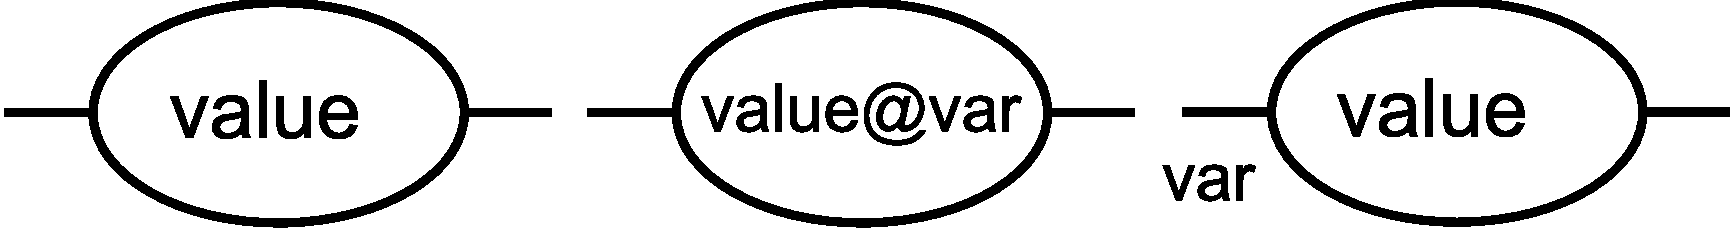
\includegraphics{images/stateVariable}
  \caption{The \PD glyph for \glyph{state variable}, shown with a value and a variable on the far left, with only a value on the middle-left, with an additional label for the variable on the middle-right (discouraged), and decorating a \glyph{macromolecule} (\sect{macromolecule}) on the far right.}
  \label{fig:state-var}
\end{figure}

\begin{figure}[H]
  \centering
    \begin{tabular}{lc}
        A & \raisebox{-\height}{\includegraphics{examples/wrongStateVariablesA}}\\
        B & \raisebox{-\height}{\includegraphics{examples/wrongStateVariablesB}}
    \end{tabular}
  \caption{A. Examples of discouraged use of \glyph{state variables}. B. Encouraged use.}
 \label{fig:wrong-state-var}
\end{figure}

% The following is for [X]Emacs users.  Please leave in place.
% Local Variables:
% TeX-master: "../sbgn_PD-level1"
% End:

